\section{Графики задачи}
1. Построить график квадратного трёхчлена $y=3x^2+(a+3)x+a,$ если известно,
что его корни $x_1,\ x_2$ связаны соотношением $\cfrac{1}{x_1}+\cfrac{1}{x_2}=2.$\\
2. Построить график квадратного трёхчлена $y=3x^2+(a-1)x+a,$ если известно,
что его корни $x_1,\ x_2$ связаны соотношением $\cfrac{1}{x_1}+\cfrac{1}{x_2}=-2.$\\
3. Построить график функции $y=\cfrac{x^2+3x}{|x+3|}+x.$\\
4. Построить график функции $y=\cfrac{2x-x^2}{|x-2|}+x.$\\
5. Построить график квадратного трёхчлена $y=x^2-15x+q,$ если известно,
что его корни $x_1,\ x_2$ связаны соотношением $\cfrac{1}{x_1}+\cfrac{1}{x_2}=\cfrac{5}{12}.$\\
6. Построить график квадратного трёхчлена $y=x^2+9x+q,$ если известно,
что его корни $x_1,\ x_2$ связаны соотношением $\cfrac{1}{x_1}+\cfrac{1}{x_2}=-\cfrac{1}{2}.$\\
7. Построить график функции $y=\cfrac{|x+1|}{x+1}(x-1).$\\
8. Построить график функции $y=\cfrac{|x-1|}{x-1}(x+1).$\\
9. Построить график квадратного трёхчлена $y=x^2-8x+q,$ если сумма квадратов его корней равна 34.\\
10. Построить график квадратного трёхчлена $y=x^2-8x+q,$ если квадрат разности его корней равен 4.\\
11. Построить график функции $y=\cfrac{x^2+2x+1}{|x+1|}.$\\
12. Построить график функции $y=\cfrac{x^2-2x+1}{|x-1|}.$\\
13. Построить график функции $y=\cfrac{2x^2-5x+2}{x-2}\cdot(x+1).$\\
14. Построить график функции $y=\cfrac{2x^2+5x+2}{x+2}\cdot(x-1).$\\
15. Построить график функции $y=\cfrac{x^2-5x+6}{|x-2|}.$\\
16. Построить график функции $y=\cfrac{x^2+5x+6}{|x+2|}.$\\
17. На координатной плоскости изобразите множество точек, задаваемых уравнением:\\ $(y-2x)\left(|x|-5-y\right)=0.$\\
18. Упростить и построить график $f(x)=\cfrac{\sqrt{1+\left(\cfrac{x^2-1}{2x}\right)^2}}{(x^2+1)\cdot\cfrac{1}{x}}.$\\
19. Построить график функции $y=2x^2-ax-a,$ если известно, что корни квадратного трёхчлена удовлетворяют условию $\cfrac{x_1}{x_2}+\cfrac{x_2}{x_1}=-3,5.$\\
20. Изобразить на координатной плоскости множество точек, координаты которых удовлетворяют условию $|y|=x+1.$\\
21. Изобразить на координатной плоскости множество точек, координаты которых удовлетворяют условию $|y|=x-1.$\\
22. Построить график $y=|x|+|x+2|.$\\
23. Построить график $y=|x|+|x-2|.$\\
24. Прямая проходит через точку $A(1;2)$ и пересекает ось ординат в точке, удалённой от начала координат на 2. Найти уравнение прямой.\\
25. Прямая проходит через точку $A(-1;2)$ и пересекает ось ординат в точке, удалённой от начала координат на 2. Найти уравнение прямой.\\
26. Построить график функции $y=\cfrac{x^3-2x^2-5x+6}{x+2}.$\\
27. Построить график функции $y=\cfrac{x^3+2x^2-5x-6}{x-2}.$\\
28. Построить график $y=\cfrac{x^2-3x+2}{|x-2|}.$\\
29. Построить график $y=\cfrac{x^2-4x+3}{|x-3|}.$\\
30. Найти уравнение прямой с угловым коэффициентом $k=3,$ проходящей через точку $A(1;2).$\\
31. Найти уравнение прямой с угловым коэффициентом $k=3,$ проходящей через точку $A(2;4).$\\
32. Построить график $y=1-|x-2|.$\\
33. Построить график $y=1-|x+2|.$\\
34. Найти уравнение прямой проходящей через точку $A(2;3)$ и отсекающей на осях координат равные по длине отрезки.\\
35. Найти уравнение прямой проходящей через точку $A(3;2)$ и отсекающей на осях координат равные по длине отрезки.\\
36. Постройте график функции $y=\cfrac{x^2-x-20}{x-5}.$\\
37. Постройте график функции $y=\cfrac{x^2-x-2}{x-2}.$\\
38. Построить график $y=\cfrac{(x+1)(x-3)}{|x-1|+2}.$\\
39. Построить график $y=\cfrac{(x-1)(x-3)}{|x-2|+1}.$\\
40. Найти уравнение прямых, проходящих через точку $A(0;2)$ и отсекающих прямоугольный треугольник площадью 4 с катетами, лежащими на осях координат.\\
41. Найти уравнение прямых, проходящих через точку $A(0;3)$ и отсекающих прямоугольный треугольник площадью 9 с катетами, лежащими на осях координат.\\
42. Построить график $|y|=|x-2|.$\\
43. Построить график $|y|=|x-1|.$\\
44. Найдите координаты точки, через которую проходят все прямые вида $y-2=kx-k.$\\
45. Найдите координаты точки, через которую проходят все прямые вида $y+2=kx+k.$\\
46. Известно, что парабола проходит через точку $A(-1;0,75),$ и её вершина находится в начале координат. Найдите уравнение этой параболы и вычислите, в каких точках она пересекает прямую $y=12.$\\
47. Постройте график $y=|x-2|+|x+1|.$\\
48. Прямая проходит через точку $B(2;1)$ и пересекает ось абсцисс в точке, удалённой от начала координат на 3. Напишите уравнение этой прямой.\\
49. Построить график функции $y=\sqrt{1-4x+4x^2}-3.$\\
50. Построить график функции $y=\sqrt{1+4x+4x^2}-3.$\\
51. При каких значениях $k$ прямая $y=kx$ имеет единственную общую точку
с графиком функции $y=(x-1)^2?$\\
52. При каких значениях $k$ прямая $y=kx$ имеет единственную общую точку
с графиком функции $y=(x+1)^2?$\\
53. Найти уравнение прямой, проходящей через точки $A(1;3)$ и $B(3;7).$\\
54. Найти уравнение прямой, проходящей через точки $A(2;5)$ и $B(4;9).$\\
55. Нарисовать на плоскости множество точек, удовлетворяющих условию
$\cfrac{(x^2-4)(y-x+1)}{x-2}=0.$\\
56. Нарисовать на плоскости множество точек, удовлетворяющих условию
$\cfrac{(x^2-9)(y-x+1)}{x-3}=0.$\\
57. При каких значениях $k$ прямая $y=2x-3$ имеет с параболой $y=(x-k)^2$ хотя бы одну общую точку?\\
58. При каких значениях $k$ прямая $y=2x+3$ имеет с параболой $y=(x-k)^2$ хотя бы одну общую точку?
\newpage
\noindent59. На одном из рисунков изображён график функции $f(x)=2(x-1)^4+1.$ Укажите на каком и обоснуйте свой выбор.\\
\begin{tikzpicture}[scale=0.5]
\begin{axis}[
    axis lines = middle,
    legend pos={south west},
    %xlabel = {$x$},
    %xlabel style={below right},
    %ylabel = {$y$},
    title={$\text{Рис. 1}$},
    ymin=-0.5,
    ymax=3.8
               ]
	\addplot[domain=-2:3, samples=100, color=black] {2*(x-1)^4+1};
	%\addlegendentry{$\text{Рис. 1}$};
\end{axis}
\draw (0.5,5.7) node {\tiny $y$};
\draw (7,1) node {\tiny $x$};
\end{tikzpicture}
\begin{tikzpicture}[scale=0.5]
\begin{axis}[
    axis lines = middle,
    legend pos={south west},
    %xlabel = {$x$},
    %xlabel style={below right},
    %ylabel = {$y$},
    title={$\text{Рис. 2}$},
    ymin=-1.5,
    ymax=3.8
]
	\addplot[domain=-0.5:3, samples=100, color=black] {4*(x-1)^2-1};
	%\addlegendentry{$\text{Рис. 1}$};
\end{axis}
\draw (0.5,5.7) node {\tiny $y$};
\draw (7,2) node {\tiny $x$};
\end{tikzpicture}
\begin{tikzpicture}[scale=0.5]
\begin{axis}[
    axis lines = middle,
    legend pos={south west},
    %xlabel = {$x$},
    %xlabel style={below right},
    %ylabel = {$y$},
    title={$\text{Рис. 3}$},
    ymin=-0.5,
    ymax=4.2
]
	\addplot[domain=-0.5:3, samples=100, color=black] {3*abs(x-1)+1};
	%\addlegendentry{$\text{Рис. 1}$};
\end{axis}
\draw (0.5,5.7) node {\tiny $y$};
\draw (7,1) node {\tiny $x$};
\end{tikzpicture}
\begin{tikzpicture}[scale=0.5]
\begin{axis}[
    axis lines = middle,
    legend pos={south west},
    %xlabel = {$x$},
    %xlabel style={below right},
    %ylabel = {$y$},
    title={$\text{Рис. 4}$},
    ymin=-0.5,
    ymax=4.2
]
	\addplot[domain=-0.5:7, samples=100, color=black] {(x^2-6*x)*0.2+3};
	%\addlegendentry{$\text{Рис. 1}$};
\end{axis}
\draw (1,5.7) node {\tiny $y$};
\draw (7,1) node {\tiny $x$};
\end{tikzpicture}\\
60. На одном из рисунков изображён график функции $f(x)=1-3(x+1)^4.$ Укажите на каком и обоснуйте свой выбор.\\
\begin{tikzpicture}[scale=0.5]
\begin{axis}[
    axis lines = middle,
    legend pos={south west},
    %xlabel = {$x$},
    %xlabel style={below right},
    %ylabel = {$y$},
    title={$\text{Рис. 1}$},
    ymin=-3.5,
    ymax=1.2,
    xmin=-2.5,
    xmax=1.5
               ]
	\addplot[domain=-3.5:0.5, samples=100, color=black] {1-3*(x+1)^4};
	%\addlegendentry{$\text{Рис. 1}$};
\end{axis}
\draw (4.8,5.7) node {\tiny $y$};
\draw (7,4) node {\tiny $x$};
\end{tikzpicture}
\begin{tikzpicture}[scale=0.5]
\begin{axis}[
    axis lines = middle,
    legend pos={south west},
    %xlabel = {$x$},
    %xlabel style={below right},
    %ylabel = {$y$},
    title={$\text{Рис. 2}$},
    ymin=-3.5,
    ymax=0.5
]
	\addplot[domain=-3.5:0.5, samples=100, color=black] {-x^2-2*x-2};
	%\addlegendentry{$\text{Рис. 1}$};
\end{axis}
\draw (5.5,5.7) node {\tiny $y$};
\draw (7,5.5) node {\tiny $x$};
\end{tikzpicture}
\begin{tikzpicture}[scale=0.5]
\begin{axis}[
    axis lines = middle,
    legend pos={south west},
    %xlabel = {$x$},
    %xlabel style={below right},
    %ylabel = {$y$},
    title={$\text{Рис. 3}$},
    ymin=-3.5,
    ymax=1.5
]
	\addplot[domain=-2.5:0.5, samples=100, color=black] {-4*abs(x+1)+1};
	%\addlegendentry{$\text{Рис. 1}$};
\end{axis}
\draw (6.1,5.7) node {\tiny $y$};
\draw (7,3.5) node {\tiny $x$};
\end{tikzpicture}
\begin{tikzpicture}[scale=0.5]
\begin{axis}[
    axis lines = middle,
    legend pos={south west},
    %xlabel = {$x$},
    %xlabel style={below right},
    %ylabel = {$y$},
    title={$\text{Рис. 4}$},
    ymin=-2.5,
    ymax=1.5
]
	\addplot[domain=-5:0.5, samples=100, color=black] {-0.33*x*x-2*x-2};
	%\addlegendentry{$\text{Рис. 1}$};
\end{axis}
\draw (6.1,5.7) node {\tiny $y$};
\draw (7,4) node {\tiny $x$};
\end{tikzpicture}\\
61. Постройте график функции $y=\cfrac{3x^2-8x+4}{|2x-2|-x}.$ При каких $a$ прямая $y=a$ не имеет с графиком общих точек?\\
62. Постройте график функции $y=\cfrac{3x^2+8x+4}{|2x+2|+x}.$ При каких $a$ прямая $y=a$ не имеет с графиком общих точек?\\
63. Вычислите площадь треугольника, ограниченного графиком функции $y=|2x-2|-1$ и осью абсцисс.\\
64. Вычислите площадь треугольника, ограниченного графиком функции $y=|2x+2|-1$ и осью абсцисс.\\
65. На координатной плоскости изображены графики функций $y=-(x^2-9)(x^2-4)(x-1)(x-2)+10x-10x^2$ и $y=70|1-2||x|-2||-10x^2+10x-70$ при
$x\in[-3,1;2,5].$\\
a. Установите, график какой из функций синий, а какой --- красный. Ответ обоснуйте.\\
b. Решите неравенство  $-(x^2-9)(x^2-4)(x-1)(x-2)+10x-10x^2 >70|1-2||x|-2||-10x^2+10x-70$ при
$x\in[-3;2,5]$ и запишите ответ (обоснование не требуется).
\begin{center}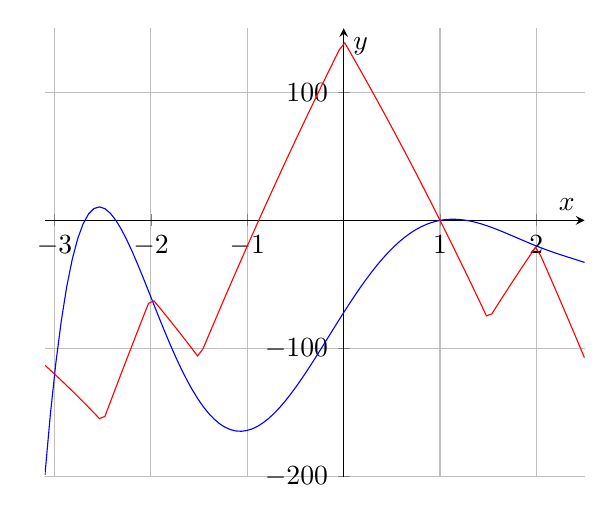
\begin{tikzpicture}[scale=1]
\begin{axis}[
    axis lines = middle,
    grid=major,
    legend pos={south west},
    xlabel = {$x$},
    %xlabel style={below right},
    ylabel = {$y$},
    ymin=-200,
    ymax=150
               ]
	\addplot[domain=-3.1:2.5, samples=100, color=blue] {-(x^2-9)*(x^2-4)*(x-1)*(x-2)+10*x-10*x^2};
\addplot[domain=-3.1:2.5, samples=100, color=red] {70*abs(1-2*abs(abs(x)-2))-10*x^2+10*x-70};
	%\addlegendentry{$\text{Рис. 1}$};
\end{axis}
\end{tikzpicture}\end{center}
66. На координатной плоскости изображены графики функций $y=(x^2-9)(x^2-4)(x-1)(x-2)+7x-12x^2$ и $y=-50(|1-|2|x|-4||-1)+7x-12x^2$ при
$x\in[-2,5;3,1].$\\
a. Установите, график какой из функций синий, а какой --- красный. Ответ обоснуйте.\\
b. Решите неравенство  $-50(|1-|2|x|-4||-1)+7x-12x^2 >(x^2-9)(x^2-4)(x-1)(x-2)+7x-12x^2$ при
$x\in[-2,5;3]$ и запишите ответ (обоснование не требуется).
\begin{center}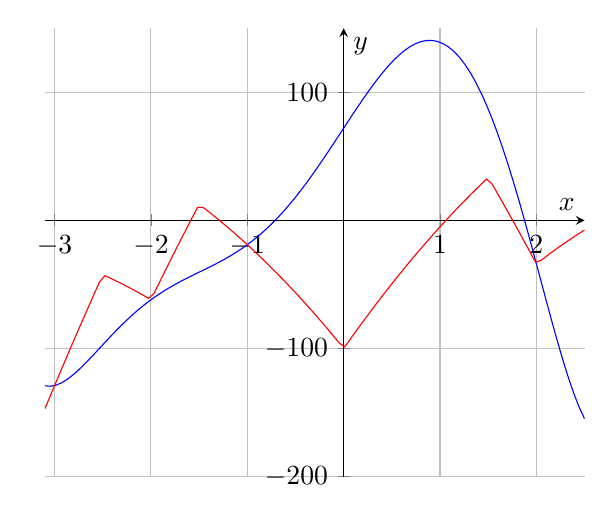
\begin{tikzpicture}[scale=1]
\begin{axis}[
    axis lines = middle,
    grid=both,
    legend pos={south west},
    xlabel = {$x$},
    %xlabel style={below right},
    ylabel = {$y$},
    ymin=-200,
    ymax=150
               ]
	\addplot[domain=-3.1:2.5, samples=100, color=blue] {(x^2-9)*(x^2-4)*(x+1)*(x+2)+7*x-12*x^2};
\addplot[domain=-3.1:2.5, samples=100, color=red] {-50*(abs(1-abs(2*abs(x)-4))-1)+7*x-12*x^2};
	
\end{axis}
\end{tikzpicture}\end{center}
67. а) Построить график функции $f(x)=x\cdot|4-x|.$\\
б) При каких значениях параметра $a$ уравнение $ax-2=x\cdot|4-x|$ имеет ровно два решения?\\
68. а) Построить график функции $f(x)=x^2-2|x|.$\\
б) При каких значениях $a$ уравнение $x^2-2|x|=a$ имеет ровно три решения?\\
69. На графике $y=x^2$ найти все точки, сумма расстояний от которых до координатных осей равна 2.\\
70. Постройте график функции $y=x^2-4x-5.$ Найдите наибольшее и наименьшее значение функции на отрезке $[-1;3]$ (то есть при $-1\leqslant x \leqslant 3).$\\
71. Дана функция $f(x)=\cfrac{|x^2-x-6|\cdot(x-4)}{3-x}.$\\
а) Постройте график данной функции.\\
б) укажите все значения параметра $p,$ при которых количество корней уравнения $f(x)=p$ чётно.\\
72. а) Постройте график функции $f(x)=(x+1)|x-1|.$\\
б) Укажите промежутки возрастания, промежутки, где функция принимает положительные значения, и те значения $c,$ при которых уравнение $f(x)=c$ имеет три решения.\\
73. На графике функции $y=3x^2$ найдите все точки, расстояние от которых до прямой $y=x-2$ равно $2\sqrt{2}.$\\
74. Найдите значения параметров $a,\ b,\ c$ такие, что точка $A(0;4)$ лежит на параболе $y=ax^2+bx+c,$ а точка $N(-1;6)$ --- вершина этой параболы.\\
75. Постройте график функции $y=\sqrt{(1-2x)^2}-3$ и найдите радиус окружности, описанной около треугольника, отсекаемого осью $Ox$ от этого графика.\\
76. Найдите уравнения всех прямых, которые проходят через начало координат и имеют единственную общую точку с графиком функции $y=(x-1)^2.$\\
77. Найдите все значения $b$ такие, что функция $y=bx^2-6x+3$ имеет наименьшее значение, и это значение меньше, чем 2,5.\\
78. Парабола $y=x^2+6x+c$ пересекает ось $Oy$ в точке с ординатой $-10.$ Найдите наименьшее возможное значение $a,$ при котором прямая $y=a$ имеет хотя бы одну общую точку с этой параболой.\\
79. Изобразите множество точек $(x;y)$ координатной плоскости, для каждой из которых выполняется условие $\cfrac{x^2+y-2}{x+3}=0.$ Укажите в этом множестве все точки, равноудалённые от осей координат. Ответ полностью обоснуйте.\\
80. Построить на одном чертеже графики функций а) $y=|x-2|,$ б) $y=x^2.$\\
Указать точки пересечения обоих графиков с осями координат и между собой, если такие точки существуют.\\
81. Найти все значения параметра $a,$ при которых графики функций $y=ax^2-ax$ и $y=ax-4$ не пересекаются.\\
82. Постройте график функции $y=\cfrac{|x-1|}{x-1}(x^2-4).$\\
83. Постройте график $y=\left|\cfrac{2-x}{4}\right|.$\\
При каких значениях аргумента выполняется неравенство $-1\leqslant y<1?$\\
84. Постройте график $y=\left|\cfrac{3+x}{6}\right|.$\\
При каких значениях аргумента выполняется неравенство $-1\leqslant y\leqslant2?$\\
85. Парабола с вершиной в точке $A(0;-3)$ проходит через точку $B(6;15).$ В каких точках эта парабола пересекает ось $x?$\\
86. Парабола с вершиной в точке $C(0;5)$ проходит через точку $B(4;-3).$ В каких точках эта парабола пересекает ось $x?$\\
87. При каком $k$ графики функций $y=x^2-2x+239$ и $y=k$ пересекаются в одной точке?\\
88. При каком $k$ графики функций $y=x^2+2x-239$ и $y=k$ пересекаются в одной точке?\\
89. Найдите площадь треугольника, ограниченного осями координат и прямой $y=2x-1.$\\
90. Найдите площадь треугольника, ограниченного осями координат и прямой $y=-2x+1.$\\
91. Найдите расстояние от начала координат до прямой $y=2-2x.$\\
92. Найдите расстояние от начала координат до прямой $y=2+2x.$\\
93. Построить график $y=\cfrac{|x^2-5x+6|}{x-2}.$\\
94. Построить график $y=\cfrac{|x^2-6x+8|}{x-2}.$\\
95. На координатной плоскости изобразите множество точек $\cfrac{(x-1)(y-3)(y-2x)}{x-2}=0.$\\
96. На координатной плоскости изобразите множество точек $\cfrac{(x-2)(y-1)(y-2x)}{x-1}=0.$\\
97. Записать уравнение параболы, если известно, что она проходит через точку $(-2;5),$ а её вершиной является точка $(-1;2).$\\
98. Записать уравнение параболы, если известно, что она проходит через точку $(-1;6),$ а её вершиной является точка $(1;2).$\\
99. а) Напишите уравнение квадратичной функции, график которой проходит через точку $C(1;3)$ и пересекает ось $OX$ в точках с абсциссами 2 и $-1.$\\
б) Лежат ли точки $A(1;1),\ B(2;4)$ и $C(3;11)$ на графике одной квадратичной функции?\\
100. а) Напишите уравнение квадратичной функции, график которой проходит через точку $C(-1;3)$ и пересекает ось $OX$ в точках с абсциссами 1 и $-2.$\\
б) Лежат ли точки $A(1;1),\ B(2;4)$ и $C(3;13)$ на графике одной квадратичной функции?\\
101. На рисунке изображён график функции $y=f(x).$ При каких значениях $x$ значения функции больше 1?
\begin{figure}[ht!]
\center{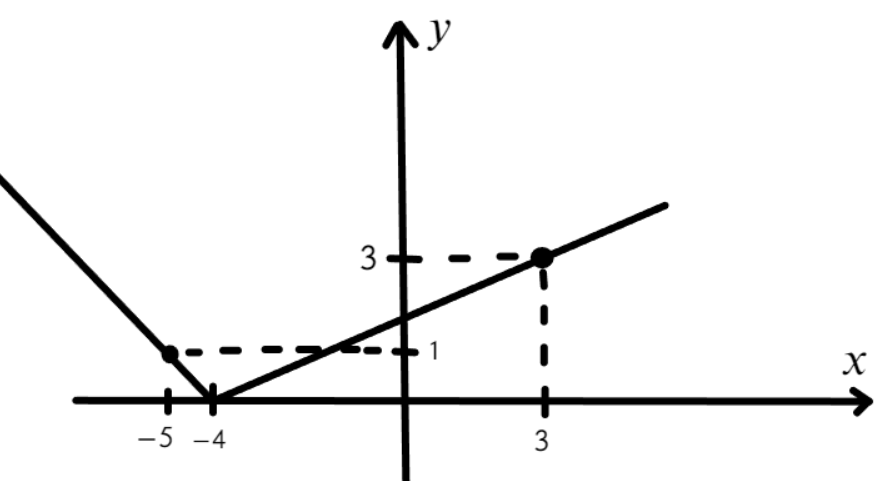
\includegraphics[scale=0.35]{gr8-101.png}}
\end{figure}\\
102. Построить множество точек, для которых выполнено условие:
$$\cfrac{(y+1)(2x^2-xy-y^2)}{x^2+xy-2y-4}=0.$$
103. а) Постройте график функции $g(x)=\cfrac{4\sqrt{x^2+4x+4}}{\sqrt{16+8x+x^2}+x}.$\\
б) С помощью построенного в предыдущем задании графика определите все значения $k,$ при каждом из которых прямая $y=k(x+2)$ имеет с данным графиком более одной общей точки.\\
104. а) Постройте график функции $g(x)=\cfrac{6\sqrt{x^2-2x+1}}{\sqrt{4-4x+x^2}-x}.$\\
б) С помощью построенного в предыдущем задании графика определите все значения $k,$ при каждом из которых прямая $y=k(x-1)$ имеет с данным графиком более одной общей точки.\\
105. Постройте график функции $y=\cfrac{2x(4x^2-1)}{2x^2-x}$ и определите, какие значения может принимать $y.$\\
106. Постройте график функции $y=\cfrac{2x(x^2-9)}{x^2-3x}$ и определите, какие значения может принимать $y.$\\
107. Изобразите множество точек, координаты которых удовлетворяют условию $(|x-2|-1)(y+x^2-2x-3)=0.$\\
108. а) Упростить выражение $\cfrac{(x^2+4x+3)(x-1)}{x+1}$ и построить график функции \\$f(x)=\cfrac{(x^2+4x+3)(x-1)}{x+1}.$\\
б) Найти все значения, которые принимает функция $f$ при $x\in[-2;1].$\\
109. Постройте график функции $\cfrac{x^2-10x+24}{|x-7|+|x-3|-2}.$\\
110. Постройте график функции $\cfrac{x^2-8x+15}{|x-6|+|x-2|-2}.$\\
111. Вершина параболы $y=f(x)$ расположена в точке $\left(\cfrac{7}{2};2\cfrac{3}{5}\right),$ а один из корней уравнения $f(x)=0$
равен $\sqrt{2}.$ Найдите второй корень.\\
112. Вершина параболы $y=f(x)$ расположена в точке $\left(\cfrac{5}{2};3\cfrac{2}{5}\right),$ а один из корней уравнения $f(x)=0$
равен $\sqrt{3}.$ Найдите второй корень.\\
113. На координатной плоскости проведены прямые $y=\cfrac{2}{3}x,\ y=4x,\ x+y=5.$ Найдите точки их пересечения и вычислите площадь треугольника
с вершинами в этих точках.\\
114. На координатной плоскости проведены прямые $y=\cfrac{4}{3}x,\ y=6x,\ x+y=7.$ Найдите точки их пересечения и вычислите площадь треугольника
с вершинами в этих точках.\\
115. Построить графики функций\\
а) $y=-x^2+4x-3;$\\
б) $y=-x^2+4|x|-3.$\\
116. Построить графики функций\\
а) $y=-x^2+2x-3;$\\
б) $y=-x^2+2|x|-3.$
\newpage
